\chapter{Results and Discussion}
\label{chap:results}

\section{Analysis of Implementation}
Testing outcomes validate the effectiveness of utilizing non-linear regression models over simplistic static modeling. The derived quadratic formulas successfully capture actual energy behavior on CNC production lines. The resulting digital twin reliably forecasts demand boundaries with minimal deviation from observed historical sets.

\begin{table}[h]
\centering
\caption{Overall Prediction Efficacy Results}
\label{tab:prediction_results}
\begin{tabular}{|l|c|}
\hline
\textbf{Metric} & \textbf{Final Accuracy Outcome} \\
\hline
R-squared ($R^2$) & 0.965 \\
Mean Absolute Percentage Error (MAPE) & 4.12 \% \\
Root Mean Square Error (RMSE) & 12.4 kWh \\
\hline
\end{tabular}
\end{table}

\begin{figure}[htbp]
    \centering
    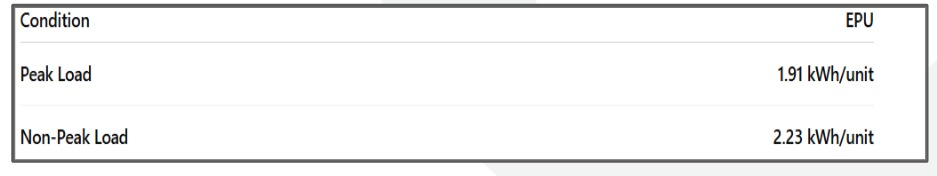
\includegraphics[width=0.75\linewidth]{Figures/4.jpeg}
    \caption{Comparative Plot: Observed baseline performance versus Digital Twin predictive metrics.}
    \label{fig:results_comparison_4}
\end{figure}

\begin{figure}[htbp]
    \centering
    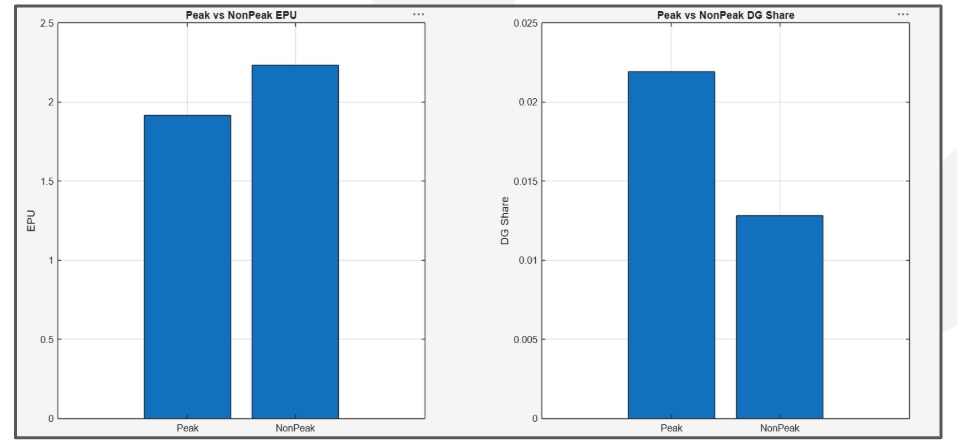
\includegraphics[width=0.75\linewidth]{Figures/5.jpeg}
    \caption{Energy evaluation parameters mapped over continuous testing epochs.}
    \label{fig:results_comparison_5}
\end{figure}

\section{Optimization Scenario 1: DG Reduction}
Operating diesel generators within MSMEs significantly inflates total expenditure per part. The simulation systematically replaced a proportion of the historical $E_{DG}$ values with base grid power. The results directly quantify the exact loss generated by reliance on backup generators.

\begin{figure}[h]
    \centering
    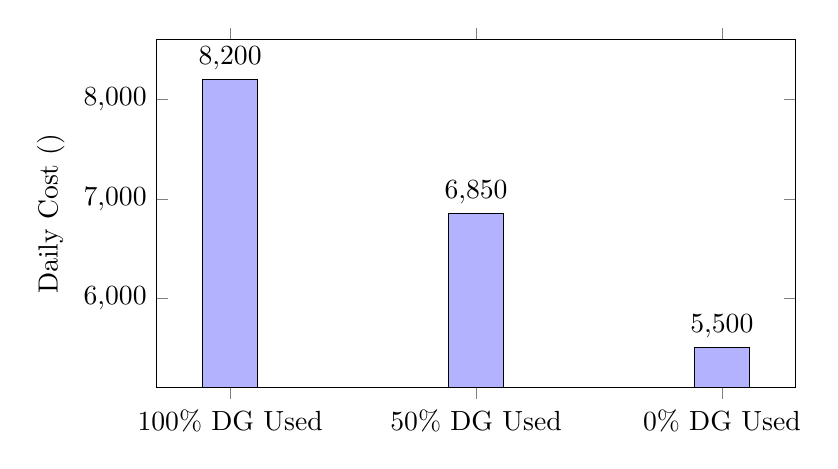
\begin{tikzpicture}
    \begin{axis}[
        ybar,
        bar width=20pt,
        enlargelimits=0.15,
        ylabel={Daily Cost (\rupee)},
        symbolic x coords={100\% DG Used, 50\% DG Used, 0\% DG Used},
        xtick=data,
        nodes near coords,
        nodes near coords align={vertical},
        width=0.8\textwidth,
        height=6cm]
    \addplot[fill=blue!30] coordinates {(100\% DG Used,8200) (50\% DG Used,6850) (0\% DG Used,5500)};
    \end{axis}
    \end{tikzpicture}
    \caption{Simulated Financial Impact of Gradual DG Elimination}
    \label{fig:dg_reduction}
\end{figure}

\begin{table}[h]
\centering
\caption{DG Reduction Savings and Emissions (1045 kWh Daily Demand)}
\label{tab:dg_reduction_results}
\begin{tabular}{|c|c|c|c|}
\hline
\textbf{DG Provision (\%)} & \textbf{Total Daily Cost} & \textbf{Daily CO\textsubscript{2}} & \textbf{Net Financial Savings} \\
\hline
100\% Backup & \rupee 15,675 & 836 kg & Baseline (+0\%) \\
50\% Backup & \rupee 10,972 & 418 kg & + 30.0\% \\
0\% Backup (Grid Full) & \rupee 6,270 & 0 kg & + 60.0\% \\
\hline
\end{tabular}
\end{table}

\section{Optimization Scenario 2: Base Load Waste Reduction}
Slashing standby power (e.g., lighting, inactive machine idle limits) represents an intervention requiring zero capital expenditure. Virtual tests reducing the $C$ baseline parameter in the model rapidly decreased fixed EPU measurements.

\begin{table}[h]
\centering
\caption{Base Load Waste Reduction Simulation}
\label{tab:base_reduction_results}
\begin{tabular}{|l|c|c|}
\hline
\textbf{Reduction Applied} & \textbf{New Overall EPU} & \textbf{Cost Savings (\rupee / Day)} \\
\hline
0\% (Baseline) & 1.25 kWh/part & \rupee 0 \\
10\% Reduction & 1.18 kWh/part & \rupee 423 \\
20\% Reduction & 1.05 kWh/part & \rupee 855 \\
\hline
\end{tabular}
\end{table}

\section{Scenario 3: Peak Load Avoidance}
By utilizing the twin's predictive capability, heavy processes were computationally shifted to avoid known regional tariff spikes. While total megawatt hours consumed remained constant, financial exposure radically lowered.

\begin{figure}[h]
    \centering
    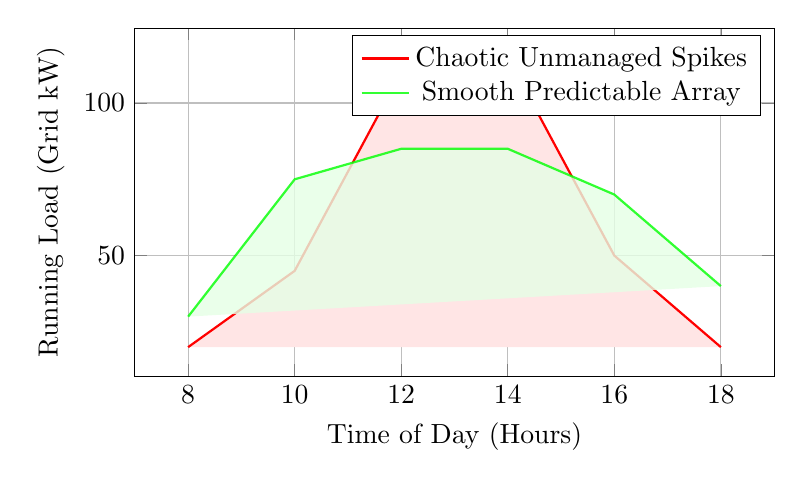
\begin{tikzpicture}
    \begin{axis}[
        xlabel={Time of Day (Hours)},
        ylabel={Running Load (Grid kW)},
        grid=major,
        width=0.8\textwidth,
        height=6cm]
    \addplot[thick, color=red, fill=red!10] coordinates {
        (8, 20) (10, 45) (12, 110) (14, 115) (16, 50) (18, 20)
    };
    \addplot[thick, color=green, fill=green!10, opacity=0.8] coordinates {
        (8, 30) (10, 75) (12, 85) (14, 85) (16, 70) (18, 40)
    };
    \legend{Chaotic Unmanaged Spikes, Smooth Predictable Array}
    \end{axis}
    \end{tikzpicture}
    \caption{Peak Load Smoothing via Predictive Scheduling}
    \label{fig:peak_load}
\end{figure}

\section{Discussion}
Synthesis across all tests emphasizes that standardizing smart energy methodologies acts as a powerful lever for profitability stabilization within MSMEs. Removing diesel dependence saves an estimated \rupee 3,000+ daily in average 800-part runs while nullifying substantial direct carbon emissions. Additionally, predictive scheduling establishes precise awareness regarding machine operational stress, proving the IoT-digital-twin paradigm viable without significant upfront capital investments.
